\chapter{Data analysis framework}
\label{chap:artframework}

\section{Offline framework for the SLAC test beam}

\ac{midas} DAQ system is developed at \ac{psi} and \ac{truimf}.

\begin{figure}[htbp]
\centering
%\fbox{\includegraphics[trim=0cm 5.5cm 0cm 5.5cm ,width=0.9\textwidth]{pics/EMShower}} guide line for trimming
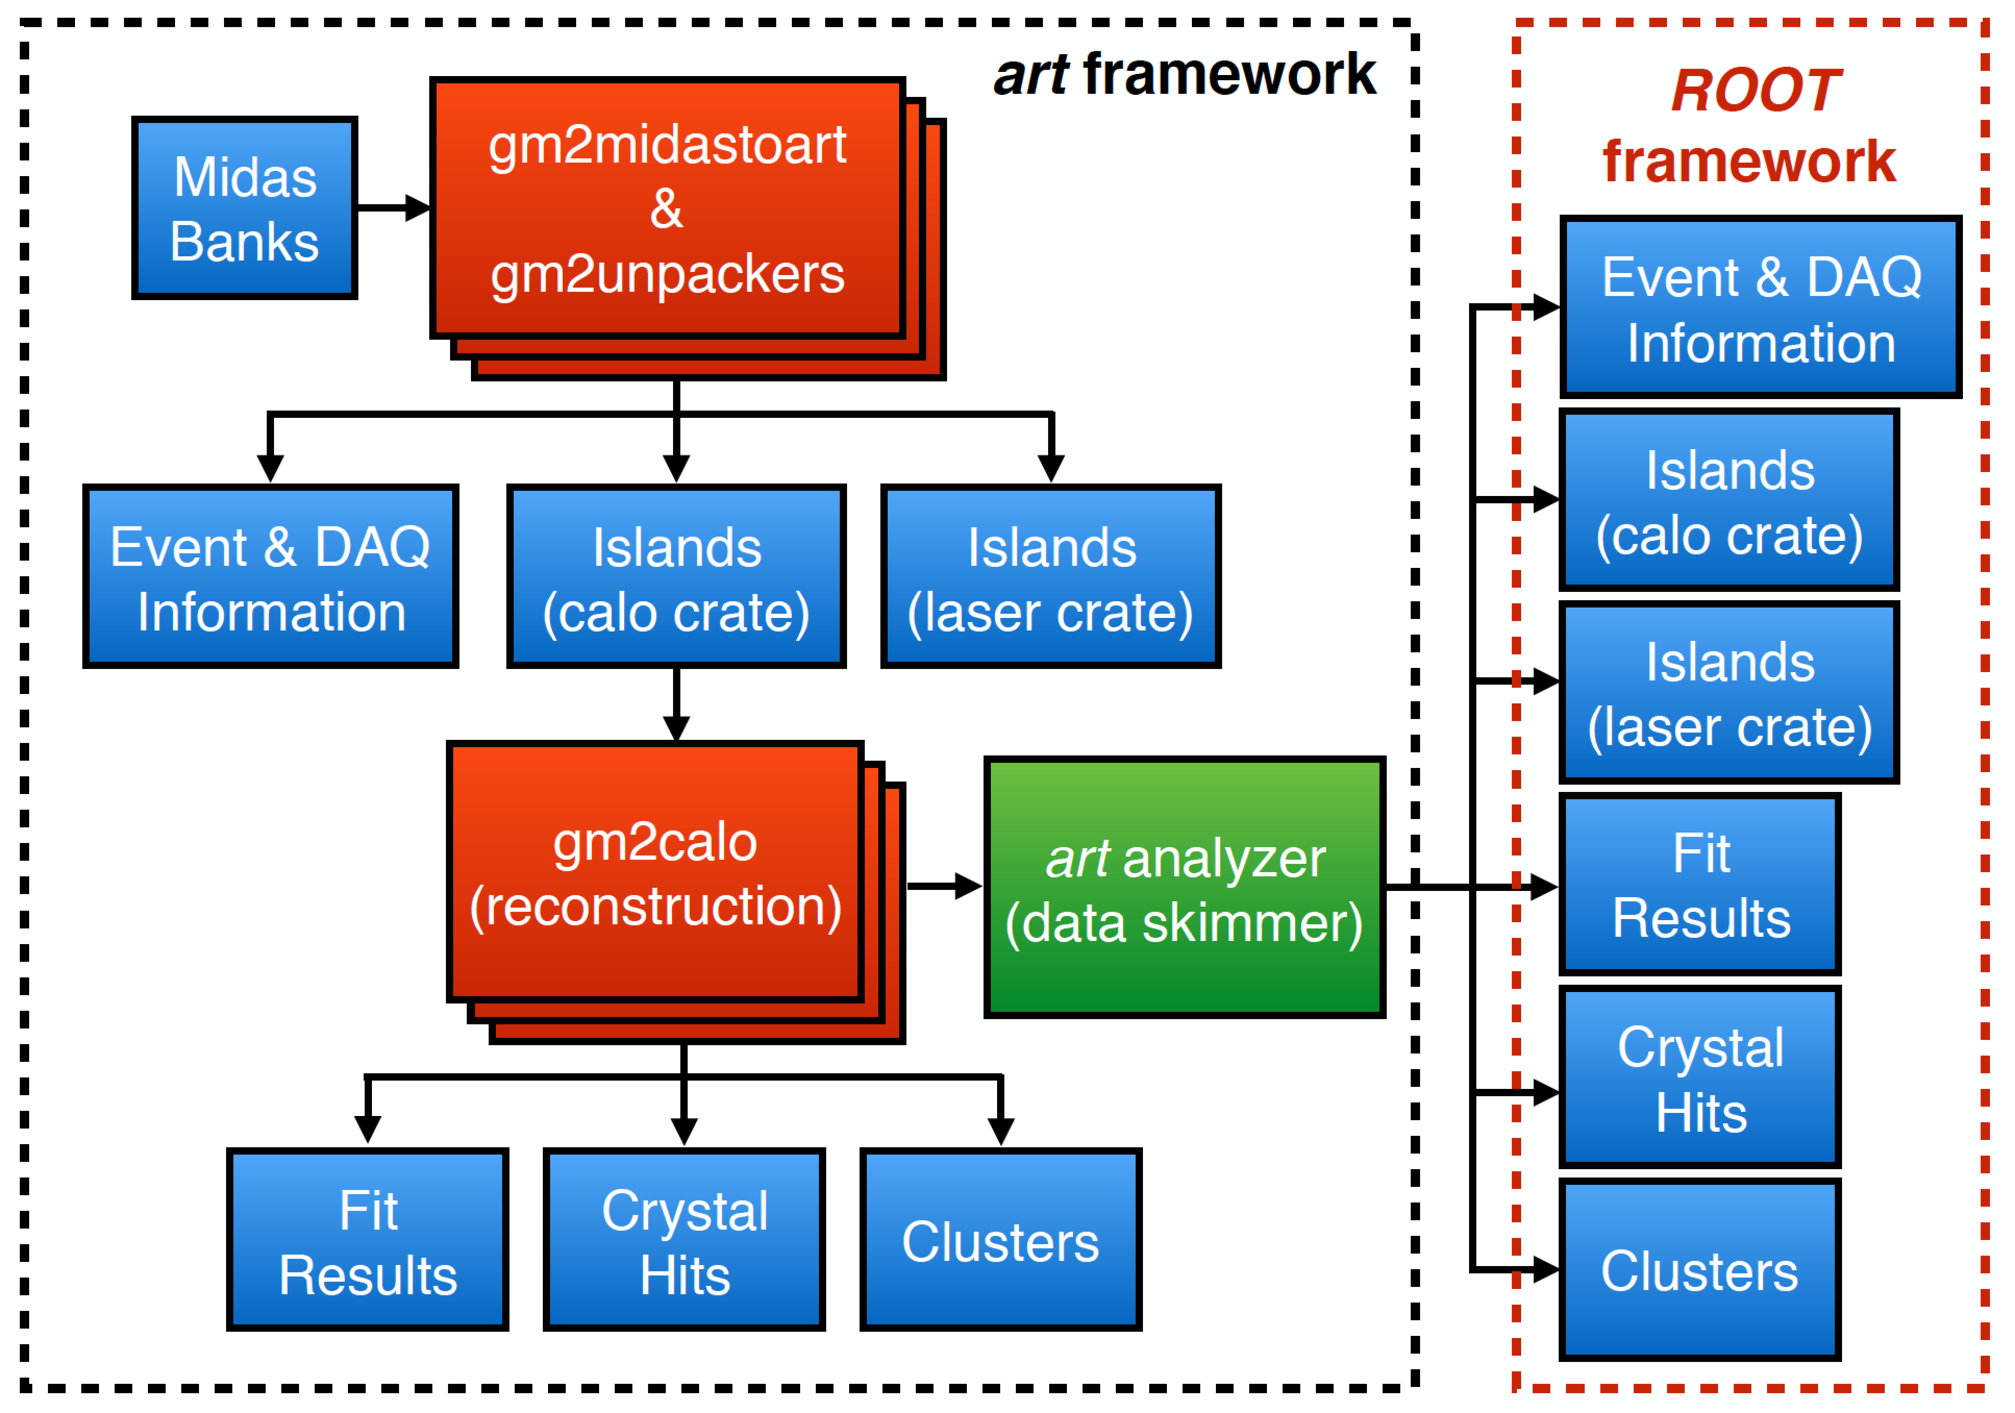
\includegraphics[width=0.8\textwidth]{pics/offline_slac_framework}
\caption{Offline framework for SLAC experimental data.}
\end{figure}

The data analysis of this test beam has several components. First we need to convert the raw data stored in a MIDAS file (\verb+.mid+ or \verb+.mid.gz+) to \textit{art} data products stored in a ROOT file.
This is handled using \textit{art} framework's modules and is doing nothing more than storing \verb+16-bit+ or \verb+32-bit+ word into \verb+vectors+. Next we unpack these \verb+vectors+
and give them contexts based on the header information stored within the \verb+vectors+. As this step, all the information are stored as data products you are probably familiar with: \verb+RiderArtRecord+,
 \verb+IslandArtRecord+, etc.

\section{Header information}
This section provides the information regarding user interface to the event, AMC13 and rider header information. All the information are stored in the art/ROOT files and standalone ROOT files with the TBranch structures in the following sections.

\section{Header and trailer formats}

This section compiles all the available header data formats. Please refer to \url{http://gm2-docdb.fnal.gov:8080/cgi-bin/ShowDocument?docid=3409} for more details.

\begin{figure}[htbp]
\centering
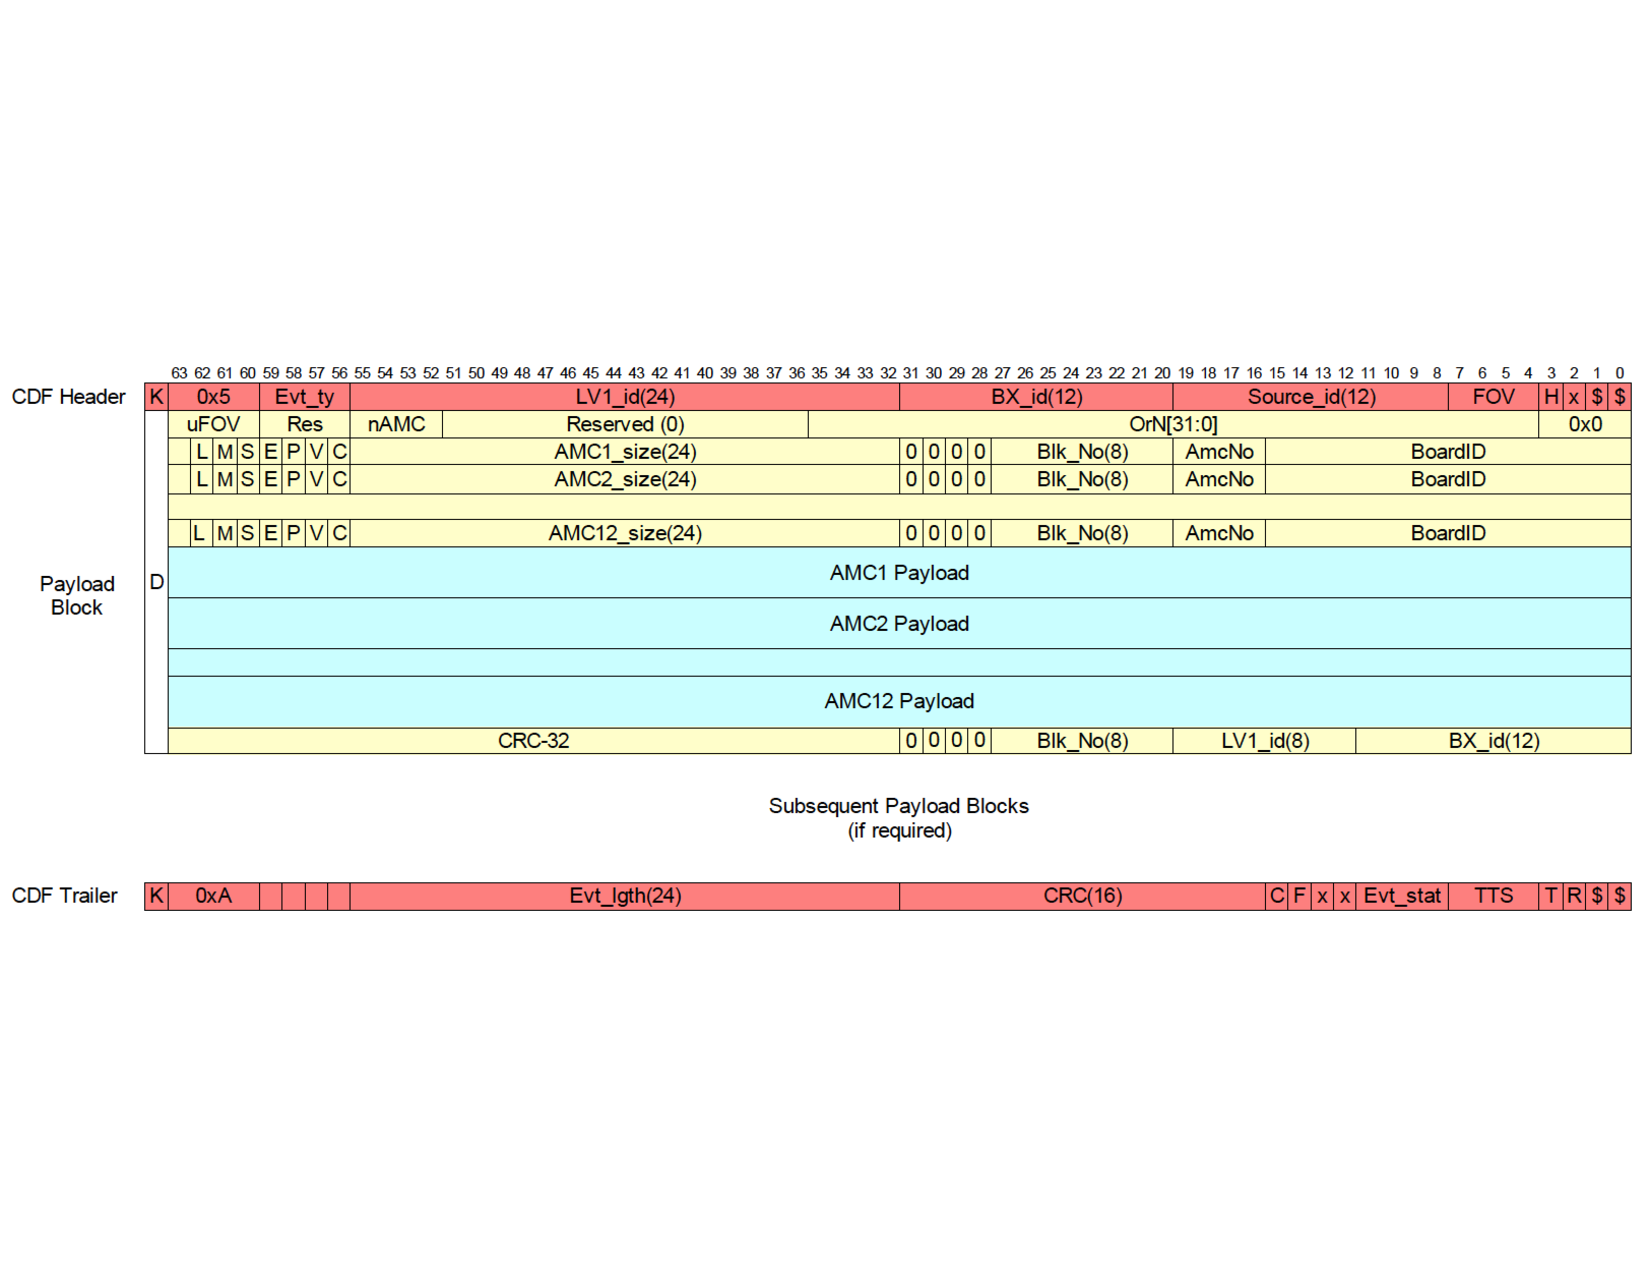
\includegraphics[trim=0cm 6cm 0cm 6cm ,width=0.95\textwidth]{pics/AMC13Header}
\caption{AMC13 to DAQ data format.}
\end{figure}

\begin{figure}[htbp]
\centering
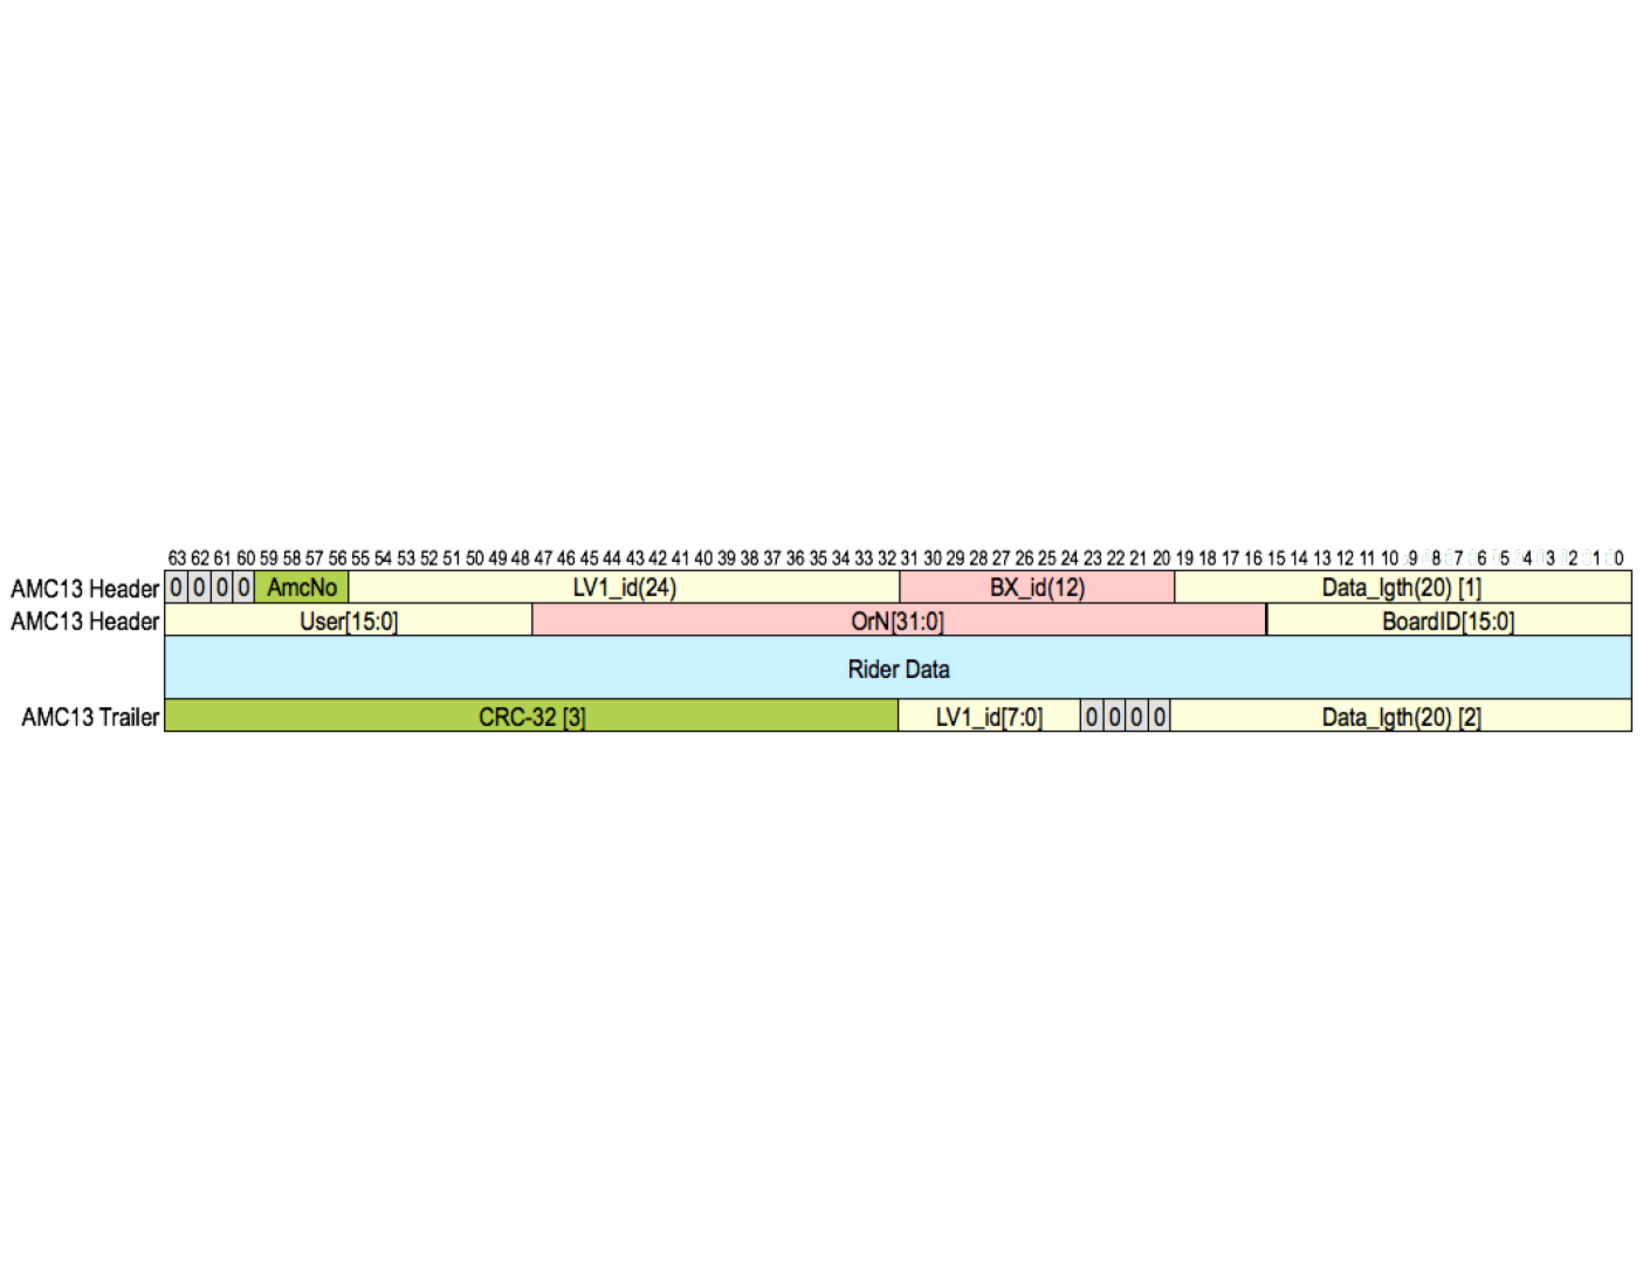
\includegraphics[trim=0cm 9.5cm 0cm 9.5cm ,width=0.95\textwidth]{pics/RiderToAMC13Header}
\caption{Rider to AMC13 data format.}
\end{figure}

%trim left bottom right top
\begin{figure}[htbp]
\centering
%\fbox{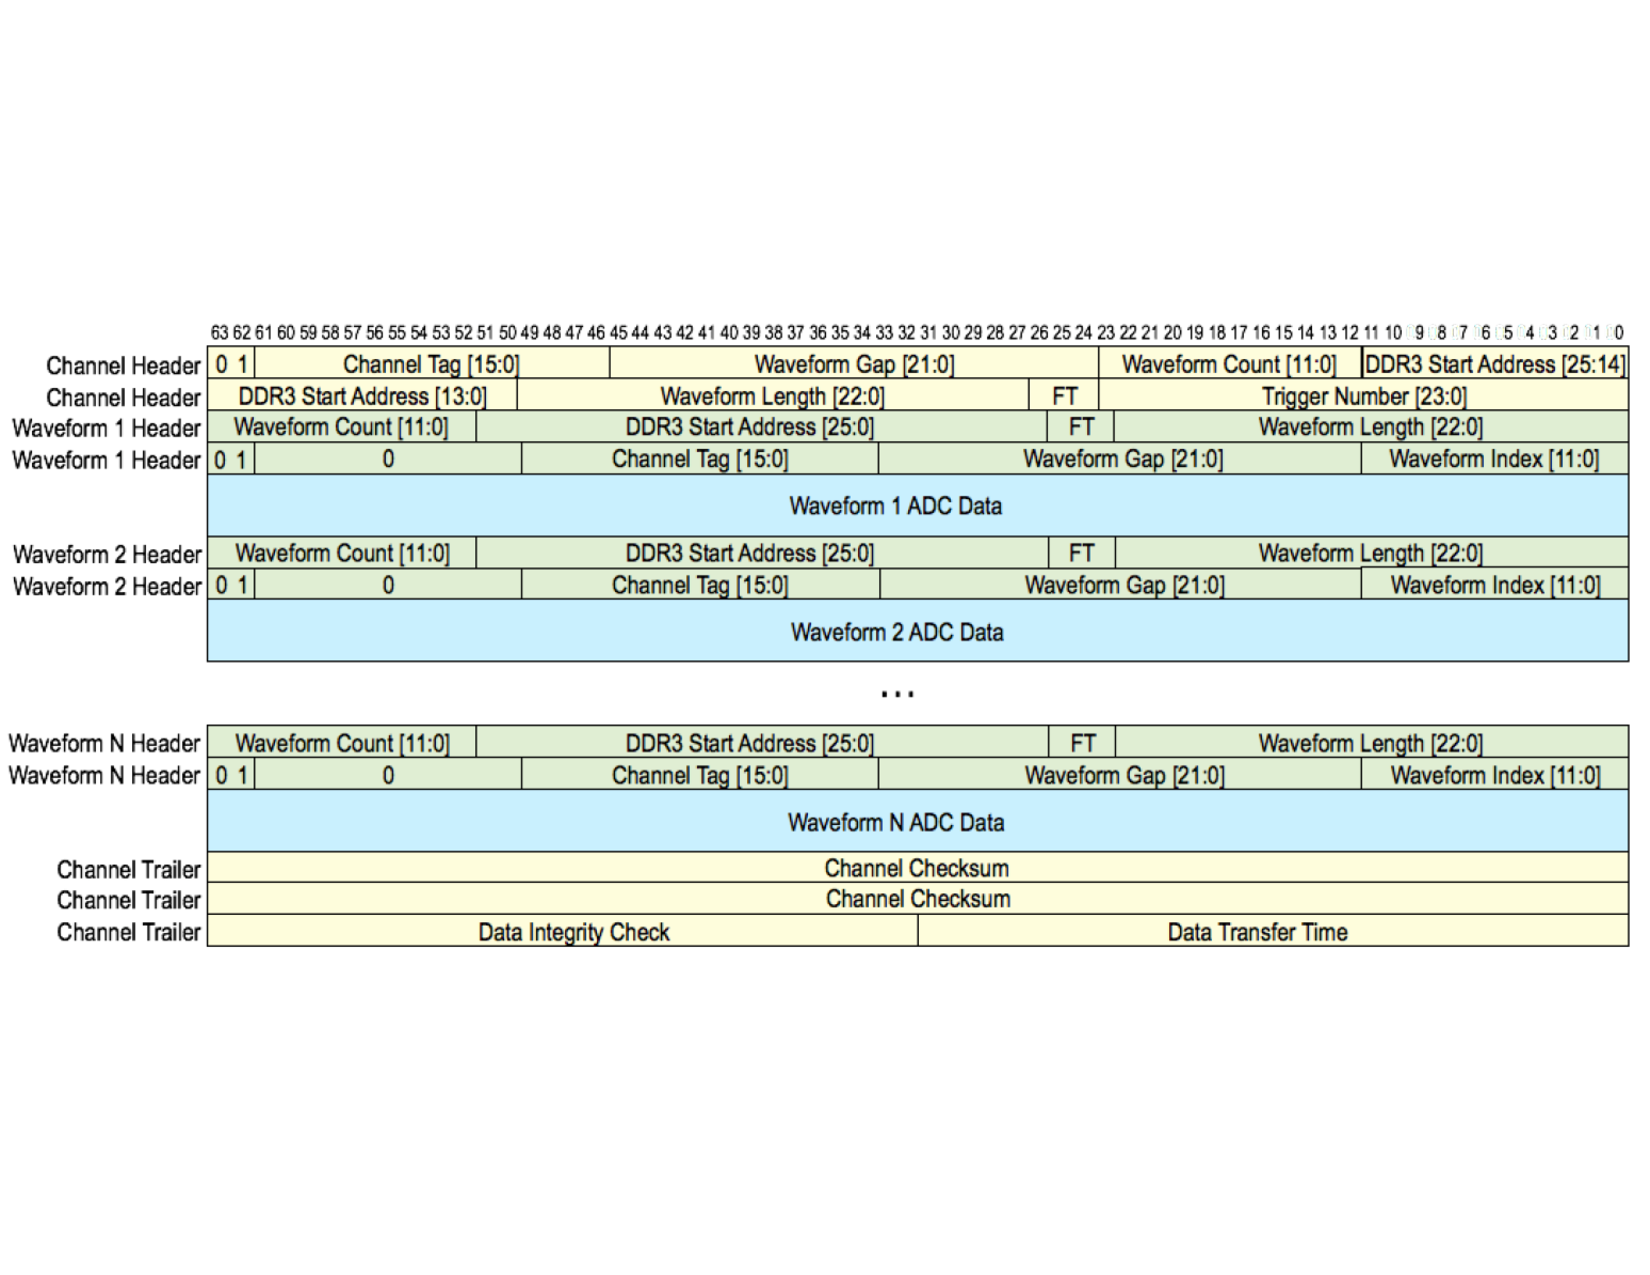
\includegraphics[trim=0cm 5.5cm 0cm 5.5cm ,width=0.9\textwidth]{pics/RiderChannelHeader}} guide line for trimming
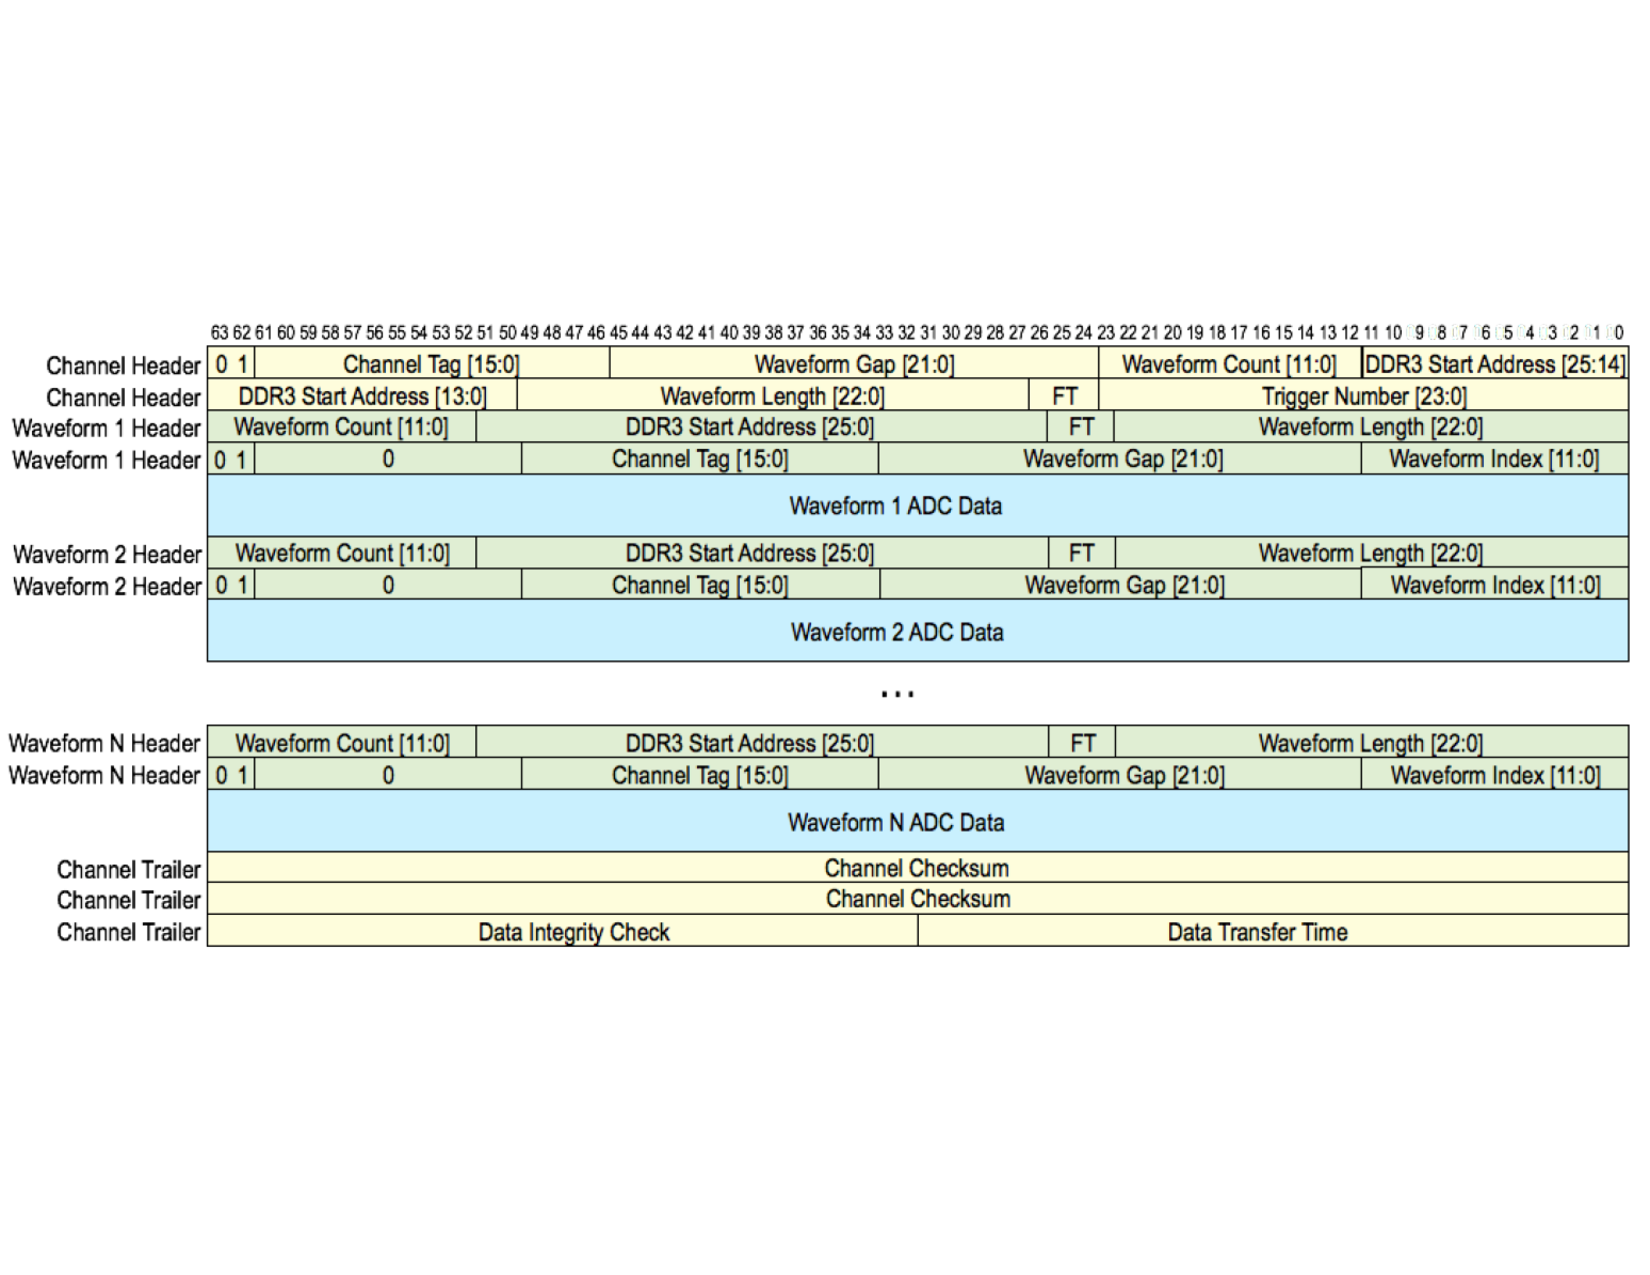
\includegraphics[trim=0cm 5.5cm 0cm 5.5cm ,width=0.95\textwidth]{pics/RiderChannelHeader}
\caption{Rider Channel data format.}
\end{figure}

\begin{figure}[htbp]
\centering
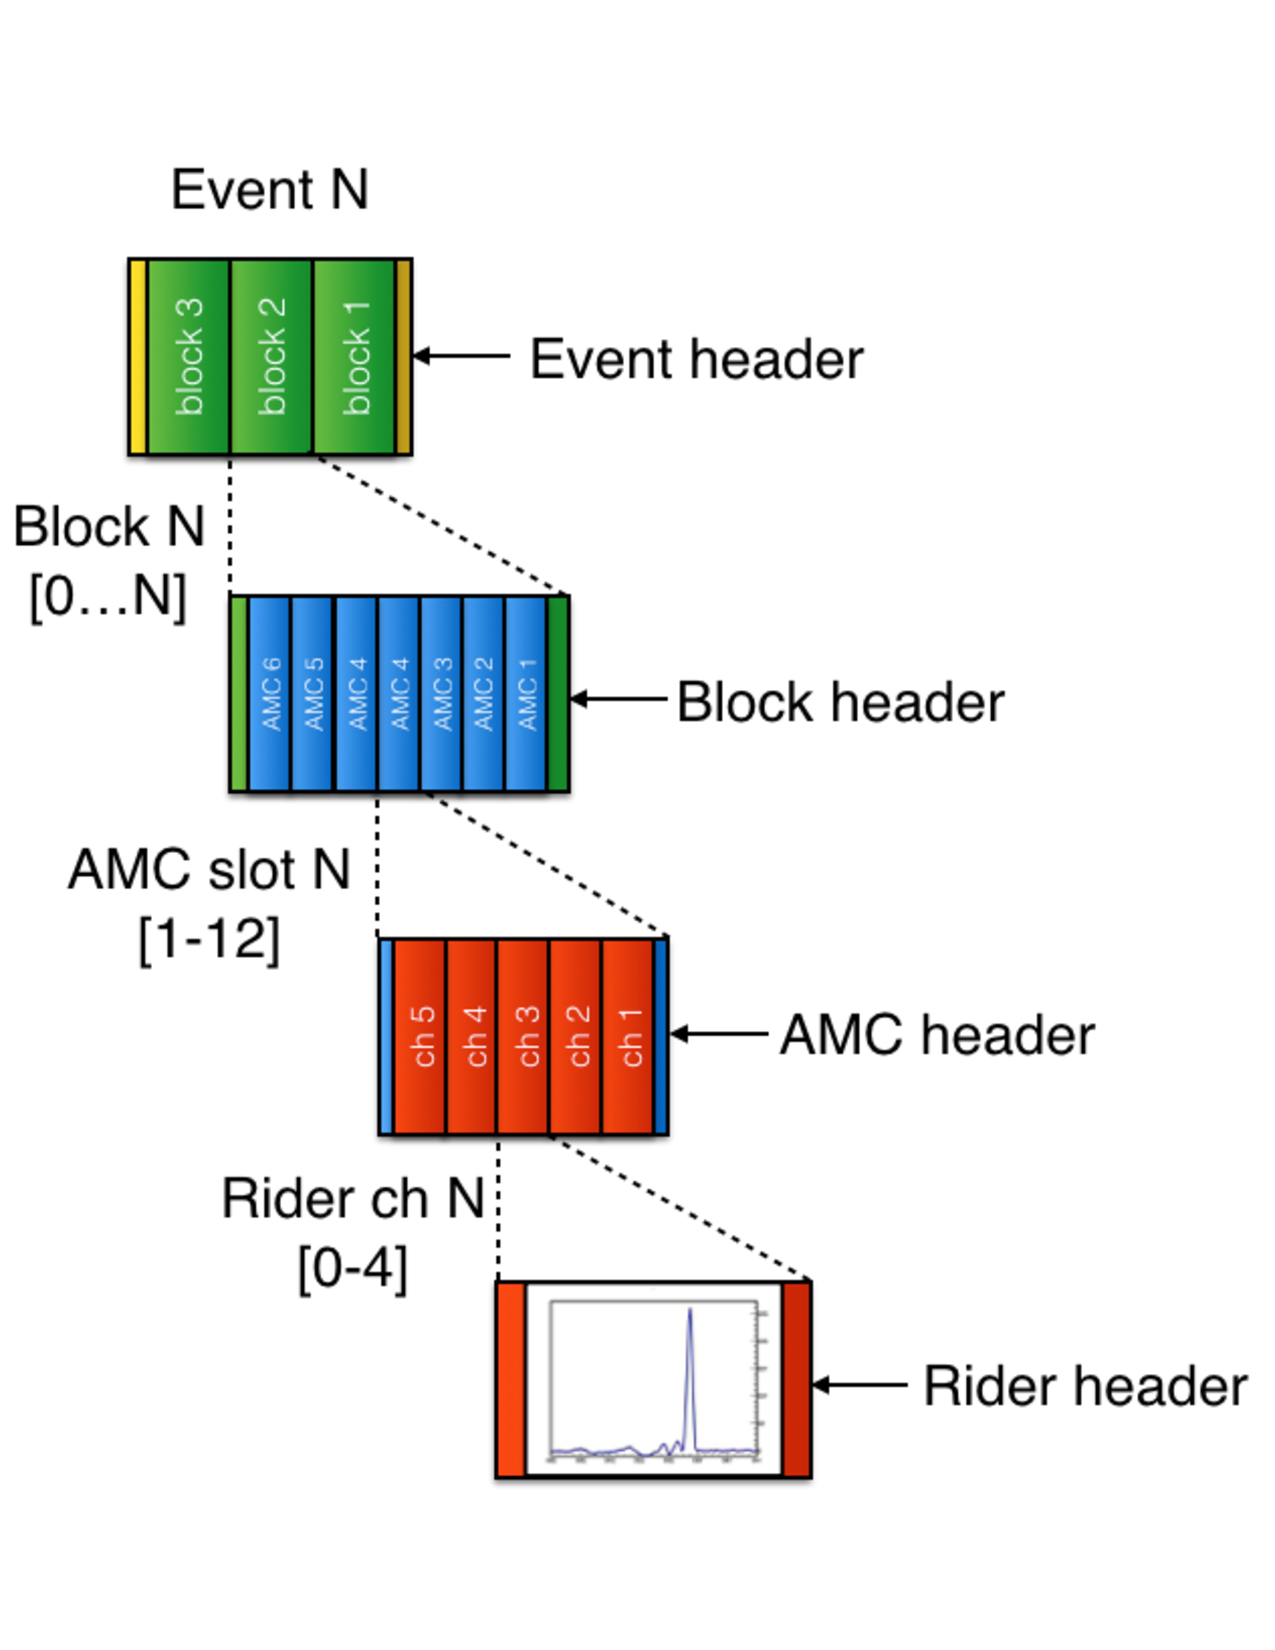
\includegraphics[width=0.9\textwidth]{pics/AllHeaders}
\caption{Per event data format}
\end{figure}


